\documentclass{beamer}

\mode<presentation> {
}

\usepackage{graphicx} % Allows including images
\usepackage{booktabs} % Allows the use of \toprule, 
\usepackage{longtable} % Allows the use of \toprule, 


\title[]{Bayesian Clinical Trials} 
\subtitle{Brief introduction to phase I and phase IIA trials} 
\date{} 


\begin{document}

\begin{frame}
\titlepage % Print the title page as the first slide
\end{frame}

\begin{frame}{Phases of drug development process}

\begin{center}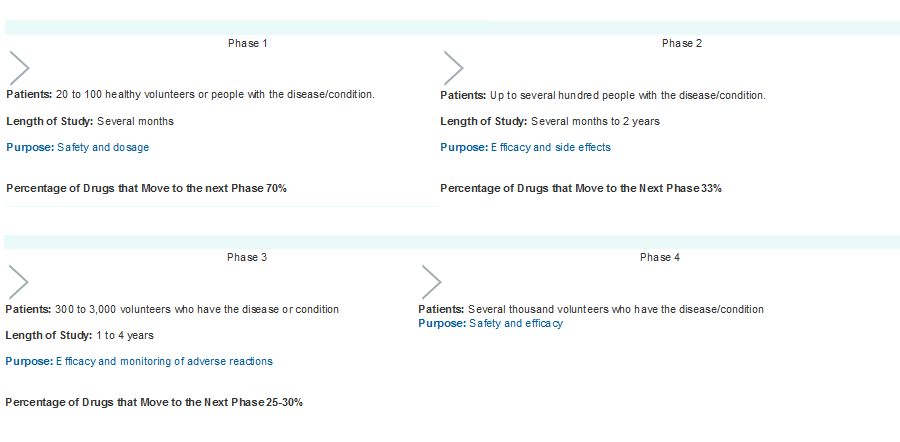
\includegraphics[scale=0.4]{images/Figure1b.png} \end{center}

\href{http://www.fda.org}{FDA}

\end{frame}

\begin{frame}{Phase I study}

\begin{itemize}
\item
  Goal: the first step in evaluating a potential new agent is to
  determine a dose having an acceptable level of toxicity.
\item
  Key elements:

  \begin{itemize}
  \itemsep1pt\parskip0pt\parsep0pt
  \item
    the starting dose \(d_{start}\)
  \item
    the dose-limiting toxicity (DLT)
  \item
    the target toxicity level (TTL)
  \item
    a dose escalation scheme consisting of

    \begin{itemize}
    \itemsep1pt\parskip0pt\parsep0pt
    \item
      a dose increment
    \item
      a dose assignment
    \item
      a cohort size
    \end{itemize}
  \end{itemize}
\end{itemize}

\end{frame}

\begin{frame}

\begin{itemize}
\item
  Dose levels have historically been chosen according to some variation
  of a Fibonacci sequence. A Fibonacci sequence is a sequence of numbers
  where each number is the sum of the two previous numbers in the
  sequence; an example is \{1,1,2,3,5,8,\ldots{}\}.
\item
  Based on dose assignment, phase I trials can be classified into
  rule-based methods and model-based methods
\end{itemize}

\end{frame}

\begin{frame}{Rule based designs}

\begin{itemize}
\itemsep1pt\parskip0pt\parsep0pt
\item
  Traditional 3+3 design

  \begin{itemize}
  \itemsep1pt\parskip0pt\parsep0pt
  \item
    If none of the first 3 patients experiences a DLT at \(d_{start}\)
    \(=>\) 3 more patients will be treated at the next higher dose level
    (\emph{escalation}).
  \item
    If 1 of the first 3 patients experiences a DLT \(=>\) 3 more
    patients will be treated at the same dose level.
  \item
    If 2 or 3 patients out of 3 experience a DLT \(=>\) 3 more patients
    will be treated at the next lower dose level (\emph{de-escalation}).
  \item
    The dose escalation/de-escalation continues but stops as soon as at
    least 2 patients experience DLTs, among a total of up to 6 patients
    (i.e.~probability of DLT at the dose¸ 33\%).
  \end{itemize}
\end{itemize}

\end{frame}

\begin{frame}{Rule based designs}

Example

\begin{longtable}[c]{@{}lllll@{}}
\toprule
Cohort & Dose 1 & Dose 2 & \emph{Dose 3} & Dose 4\tabularnewline
\midrule
\endhead
1 & 0/3 & & &\tabularnewline
2 & & 1/3 & &\tabularnewline
3 & & 0/3 & &\tabularnewline
4 & & & 1/3 &\tabularnewline
5 & & & 1/3 &\tabularnewline
\bottomrule
\end{longtable}

\end{frame}

\begin{frame}{Rule based designs}

\begin{itemize}
\itemsep1pt\parskip0pt\parsep0pt
\item
  Alternative statistical approaches are needed to make a better use of
  the complex data generated by phase I trials. Their applications
  require a close collaboration between all actors of early phase
  clinical trials (Paoletti et al, 2015).
\end{itemize}

\end{frame}

\begin{frame}{Model based}

\begin{itemize}
\itemsep1pt\parskip0pt\parsep0pt
\item
  Model-based methods for finding the MTD assume that there is a
  monotonic dose-toxicity relationship. In this approach, a
  dose-toxicity curve as well as the TTL are explicitly defined.
\item
  The goal for the phase I clinical trial is, through treating patients
  in a dose escalation fashion, to seek a suitable quantile of the
  dose-toxicity curve; specifically,a dose that will induce a
  probability of DLT at a specified TTL.
\item
  This method is most conveniently carried out under the Bayesian
  framework. Simple one- or two- parameter parametric models are often
  used to characterize the dose-toxicity relationship, with the Bayesian
  posterior distribution used to estimate the parameters.
\end{itemize}

\end{frame}

\begin{frame}{Model based}

\begin{center}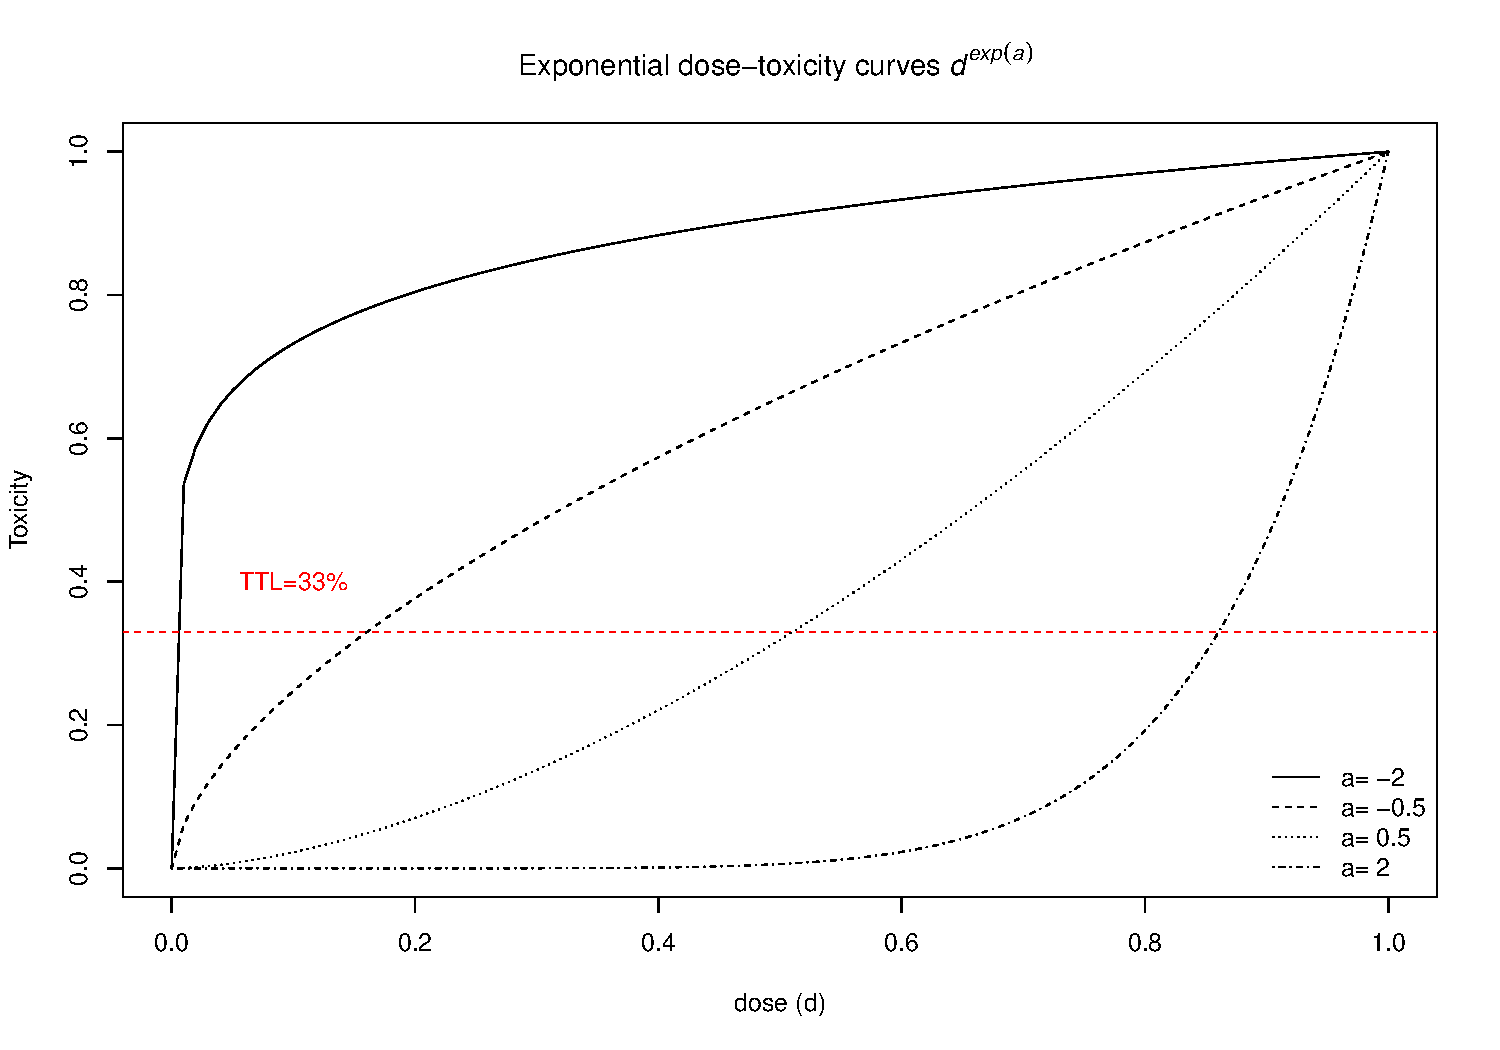
\includegraphics[scale=0.4]{indexPdf_files/figure-beamer/unnamed-chunk-1-1} \end{center}

\end{frame}

\begin{frame}{Model based}

\begin{itemize}
\item
  The continual reassessment method (CRM) seems to have been the first
  Bayesian model-based phase I design introduced in the literature
  (O'Quigley et al, 1990).
\item
  Many modifications were proposed to overcome its greatest weakness -
  i.e.~its potential for exposing patients to overly toxic doses if the
  first few patient responses are atypical or the model is misspecified
  - and its limitations such as the use of a single binary endpoint. See
  Berry et al (2011) for a review.
\end{itemize}

\end{frame}

\begin{frame}{Phase II studies}

After the toxicity profile and/or the MTD for a treatment has been
investigated, phase II studies are conducted at the MTD or an optimal
biological dose estimated from phase I.

\begin{itemize}
\itemsep1pt\parskip0pt\parsep0pt
\item
  Goal: to examine whether a drug has sufficient efficacy to warrant
  further developmentand and to refine knowledge of its toxicity
  profile.

  \begin{itemize}
  \itemsep1pt\parskip0pt\parsep0pt
  \item
    Phase IIA is single arm
  \item
    Phase IIB is multi-arm
  \end{itemize}
\end{itemize}

\end{frame}

\begin{frame}{Phase IIA designs}

To provide an initial efficacy assessment, a phase IIA trial is often
designed as a single-arm,open-label study that requires treating 40 to
100 patients in a multistage setting.

The primary endpoint is often a binary endpoint of response/no response
or success/failure.

Multi-stage designs are useful here for early stopping due to lack of
efficacy should the interim data indicate that the study drug is
inefficacious.

\end{frame}

\begin{frame}{Phase IIA designs}

\begin{itemize}
\itemsep1pt\parskip0pt\parsep0pt
\item
  Simon (1989) optimal and minimax designs:

  \begin{itemize}
  \itemsep1pt\parskip0pt\parsep0pt
  \item
    Optimal design minimize the expected sample size under the null
    hypothesis; minimax design can be constructed that minimizes the
    maximum trial sample size.\\
  \item
    After the inclusion of a pre-determined number of patients,
    \(n_{1}\), the trial is paused, and the response rate is evaluated.
  \item
    If a pre-specified minimal response rate, \(r_{1}/n_{1}\) has not
    been achieved, the treatment is not worth pursuing and the trial is
    ended.
  \item
    Otherwise, enrollment continues until a pre-determined number \(n\)
    of additional patients are accrued. The drug will be declared
    effective or ineffective depending on the achievement of an overall
    response rate\(r/n\).
  \end{itemize}
\end{itemize}

\end{frame}

\begin{frame}{Phase IIB designs}

After passing the initial efficacy assessment of a new agent in a phase
IIA study, the subsequent phase IIB trial is often a randomized,
multi-arm study.

Phase IIB trials are by definition smaller and less definitive than
phase III trials.

They use earlier endpoints, such as disease-free survival, rather than
overall survival in order to shorten study duration.

They also often have larger Type I and Type II error rates than their
phase III counterparts.

They do not yield sufficient statistical power for a head-to-head
comparison between the treatment arms.

\end{frame}

\begin{frame}{References}

\begin{itemize}
\item
  Paoletti X, Ezzalfani M, Le Tourneau C. Statistical controversies in
  clinical research: requiem for the 3 + 3 design for phase I trials.
  Ann Oncol 2015 Jun 18. pii: mdv266.
\item
  O'Quigley J, Pepe M, Fisher L. Continual reassessment method: a
  practical design for phase I clinical trials in cancer. Biometrics
  1990; 46: 33-48.
\item
  Simon R. Optimal two-stage designs for phase II clinical trials.
  Control Clin Trials 1989; 10: 1-10.
\item
  Berry S.M., Carlin B.P., Lee J.J. , Muller P. Bayesian Adaptive
  Methods for Clinical Trials. 2011 Chapman \& Hall.
\end{itemize}

\end{frame}


\end{document} 